% Font options: 10pm, 11pt, 12pt
% Align headings left instead of center: nocenter
\documentclass[xcolor=x11names,compress]{beamer}\usepackage[]{graphicx}\usepackage[]{color}
%% maxwidth is the original width if it is less than linewidth
%% otherwise use linewidth (to make sure the graphics do not exceed the margin)
\makeatletter
\def\maxwidth{ %
  \ifdim\Gin@nat@width>\linewidth
    \linewidth
  \else
    \Gin@nat@width
  \fi
}
\makeatother

\definecolor{fgcolor}{rgb}{0.345, 0.345, 0.345}
\newcommand{\hlnum}[1]{\textcolor[rgb]{0.686,0.059,0.569}{#1}}%
\newcommand{\hlstr}[1]{\textcolor[rgb]{0.192,0.494,0.8}{#1}}%
\newcommand{\hlcom}[1]{\textcolor[rgb]{0.678,0.584,0.686}{\textit{#1}}}%
\newcommand{\hlopt}[1]{\textcolor[rgb]{0,0,0}{#1}}%
\newcommand{\hlstd}[1]{\textcolor[rgb]{0.345,0.345,0.345}{#1}}%
\newcommand{\hlkwa}[1]{\textcolor[rgb]{0.161,0.373,0.58}{\textbf{#1}}}%
\newcommand{\hlkwb}[1]{\textcolor[rgb]{0.69,0.353,0.396}{#1}}%
\newcommand{\hlkwc}[1]{\textcolor[rgb]{0.333,0.667,0.333}{#1}}%
\newcommand{\hlkwd}[1]{\textcolor[rgb]{0.737,0.353,0.396}{\textbf{#1}}}%
\let\hlipl\hlkwb

\usepackage{framed}
\makeatletter
\newenvironment{kframe}{%
 \def\at@end@of@kframe{}%
 \ifinner\ifhmode%
  \def\at@end@of@kframe{\end{minipage}}%
  \begin{minipage}{\columnwidth}%
 \fi\fi%
 \def\FrameCommand##1{\hskip\@totalleftmargin \hskip-\fboxsep
 \colorbox{shadecolor}{##1}\hskip-\fboxsep
     % There is no \\@totalrightmargin, so:
     \hskip-\linewidth \hskip-\@totalleftmargin \hskip\columnwidth}%
 \MakeFramed {\advance\hsize-\width
   \@totalleftmargin\z@ \linewidth\hsize
   \@setminipage}}%
 {\par\unskip\endMakeFramed%
 \at@end@of@kframe}
\makeatother

\definecolor{shadecolor}{rgb}{.97, .97, .97}
\definecolor{messagecolor}{rgb}{0, 0, 0}
\definecolor{warningcolor}{rgb}{1, 0, 1}
\definecolor{errorcolor}{rgb}{1, 0, 0}
\newenvironment{knitrout}{}{} % an empty environment to be redefined in TeX

\usepackage{alltt}
%\documentclass[xcolor=x11names,compress,handout]{beamer}
\usepackage[]{graphicx}
\usepackage[]{color}
\usepackage{booktabs}
\usepackage{hyperref}
\usepackage{tikz}
\usepackage{multirow}
\usepackage{dcolumn}
\usepackage{bigstrut}
\usepackage{amsmath} 
\usepackage{xcolor,colortbl}
\usepackage{amssymb}
%\newcommand{\done}{\cellcolor{teal}#1}

%% Beamer Layout %%%%%%%%%%%%%%%%%%%%%%%%%%%%%%%%%%
\useoutertheme[subsection=false,shadow]{miniframes}
\useinnertheme{default}
\usefonttheme{serif}
\usepackage{Arev}
\usepackage{pdfpages}

\setbeamerfont{title like}{shape=\scshape}
\setbeamerfont{frametitle}{shape=\scshape, size=\normalsize}

\definecolor{dkblue}{RGB}{0,0,102}

\setbeamercolor*{lower separation line head}{bg=dkblue} 
\setbeamercolor*{normal text}{fg=black,bg=white} 
\setbeamercolor*{alerted text}{fg=red} 
\setbeamercolor*{example text}{fg=black} 
\setbeamercolor*{structure}{fg=black} 
 
\setbeamercolor*{palette tertiary}{fg=black,bg=black!10} 
\setbeamercolor*{palette quaternary}{fg=black,bg=black!10} 

\renewcommand{\(}{\begin{columns}}
\renewcommand{\)}{\end{columns}}
\newcommand{\<}[1]{\begin{column}{#1}}
\renewcommand{\>}{\end{column}}

\AtBeginSection{\frame{\sectionpage}}
\usepackage{xcolor}
\hypersetup{
    colorlinks,
    linkcolor={red!50!black},
    citecolor={blue!50!black},
    urlcolor={blue!80!black}
}

\setbeamertemplate{navigation symbols}{} 
\setbeamertemplate{footline}[frame number]
\setbeamertemplate{caption}{\raggedright\insertcaption\par}

\setbeamersize{text margin left=5pt,text margin right=5pt}

%%%%%%%%%%%%%%%%%%%%%%%%%%%%%%%%%%%%%%%%%%%%%%%%%%


\title{FLS 6441 - Methods III: Explanation and Causation}
\subtitle{Week 10 - Matching}
\author{Jonathan Phillips}
\date{June 2019}
\IfFileExists{upquote.sty}{\usepackage{upquote}}{}
\begin{document}




\frame{\titlepage}

\begin{frame}
\frametitle{Classification of Research Designs}
\footnotesize
\begin{table}[htbp]
  \centering
  \scalebox{0.7}{
    \begin{tabular}{|p{2.2cm}|p{5cm}|c|c|}
    \hline
          &       & \multicolumn{1}{p{2.4cm}|}{\textbf{Independence of Treatment Assignment}} & \multicolumn{1}{p{3cm}|}{\textbf{Researcher Controls Treatment Assignment?}} \bigstrut\\
    \hline
    \multicolumn{1}{|p{2.9cm}|}{\multirow{2}[4]{2.9cm}{\textbf{Controlled Experiments}}} & Field Experiments & \checkmark      & \checkmark  \bigstrut\\
\cline{2-4}          & Survey and Lab Experiments &  \checkmark     & \checkmark \bigstrut\\
    \hline
          &       &       &  \bigstrut\\
    \hline
    \multicolumn{1}{|p{2.9cm}|}{\multirow{3}[6]{2.9cm}{\textbf{Natural Experiments}}} & Natural Experiments &  \checkmark     &  \bigstrut\\
\cline{2-4}          & Instrumental Variables & \checkmark      &  \bigstrut\\
\cline{2-4}          & Discontinuities & \checkmark      &  \bigstrut\\
    \hline
          &       &       &  \bigstrut\\
    \hline
    \multicolumn{1}{|p{2.9cm}|}{\multirow{4}[8]{2.9cm}{\textbf{Observational Studies}}} & Difference-in-Differences &       &  \bigstrut\\
\cline{2-4}          & Controlling for Confounding &       &  \bigstrut\\
\cline{2-4}          & Matching &       &  \bigstrut\\
\cline{2-4}          & Comparative Cases and Process Tracing &       &  \bigstrut\\
    \hline
    \end{tabular}}%
  \label{tab:addlabel}%
\end{table}%
\normalsize
\end{frame}

\section{Matching} 

\begin{frame}
\frametitle{The Weakness of Controlling}
\begin{itemize}
\item Controlling for confounding with regression has three weak spots:
\pause
\begin{enumerate}
\item \textbf{Lack of overlap} - Extreme treated outliers alter our results, even when there are no comparable control units in the data
\pause
\item \textbf{Model-dependence} - Variable X is a confounder, but is it linear, quadratic, cubic or what? The wrong model of the real relationship with the outcome biases our results
\pause
\item \textbf{Researcher/publication bias} - Lots of freedom to tweak the regression to get positive results
\end{enumerate}
\item All of these reflect the fact that regression is \textbf{parametric}
\pause
\begin{enumerate}
\item It uses \textit{ALL} of the data
\item It requires us to specify the parameters of a model
\end{enumerate}
\end{itemize}
\end{frame}

\begin{frame}
\frametitle{The Weakness of Controlling}
\begin{itemize}
\item The solution? \pause \textbf{Non-parametric} methods for controlling for confounding
\pause
\begin{enumerate}
\item We use \textit{ONLY SOME} of the data
\item We do not specify the parameters of any model
\end{enumerate}
\pause
\item \textbf{Matching} is a non-parametric method
\pause
\begin{itemize}
\item A \textbf{pre-processing} stage 
\item Analysis of the results is separate and comes later
\end{itemize}
\end{itemize}
\end{frame}

\begin{frame}
\frametitle{Matching}
\begin{itemize}
\item If treated and control groups have the \textbf{same values} of \textbf{all} of the confounding variables, we know that treatment is independent of potential outcomes
\pause
\item There is no variation in the confounders that could possibly explain the difference between the outcomes in treated and control groups
\pause
\begin{enumerate}
\item One way of forcing balance is by \textbf{ajusting} each treated observation to predict what it would 'look like' if it were identical to a control observation - a regression model
\pause
\item An alternative is just to \textbf{throw out} all of the treated observations that do not have a comparable control observation - this is matching
\end{enumerate}
\end{itemize}
\end{frame}

\begin{frame}
\frametitle{Matching}
\begin{itemize}
\item Matching should really be called \textbf{trimming} or \textbf{pruning} 
\begin{itemize}
\item Dropping units that don't have good counterfactuals in the data
\end{itemize}
\item It succeeds only where we can measure and create balance on all confounding variables
\pause
\item Matching is \textbf{NOT} an experimental method
\end{itemize}
\end{frame}

\begin{frame}
\frametitle{Matching}
\begin{enumerate}
\item For each treated unit, find a control unit with very close values of all confounding variables, and keep both
\pause
\item Repeat for every treated unit
\pause
\item Drop all the unmatched units (eg. 'extra' treated units that are 'far away' from any control units)
\pause
\item Assess balance - re-run the matching process as many times as you can to maximize balance!
\end{enumerate}
\end{frame}

\begin{frame}
\frametitle{Matching}
\begin{enumerate}
\item For example:
\end{enumerate}
\begin{knitrout}
\definecolor{shadecolor}{rgb}{0.969, 0.969, 0.969}\color{fgcolor}
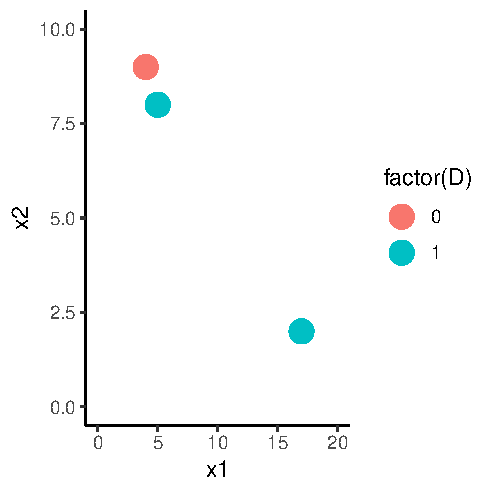
\includegraphics[width=\maxwidth]{figure/unnamed-chunk-1-1} 

\end{knitrout}
\end{frame}

\begin{frame}
\frametitle{Matching}
\begin{enumerate}
\item For example:
\end{enumerate}
\begin{knitrout}
\definecolor{shadecolor}{rgb}{0.969, 0.969, 0.969}\color{fgcolor}
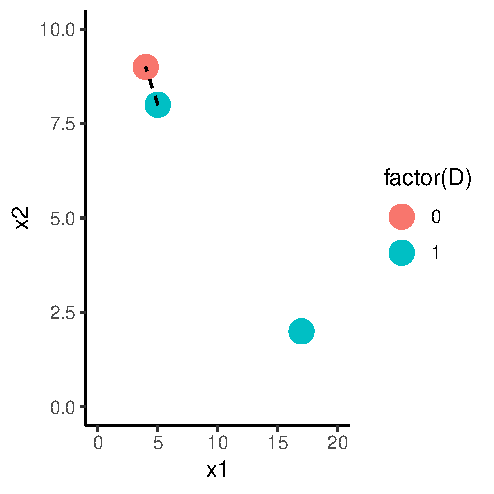
\includegraphics[width=\maxwidth]{figure/unnamed-chunk-2-1} 

\end{knitrout}
\end{frame}

\begin{frame}
\frametitle{Matching}
\begin{enumerate}
\item For example:
\end{enumerate}
\begin{knitrout}
\definecolor{shadecolor}{rgb}{0.969, 0.969, 0.969}\color{fgcolor}
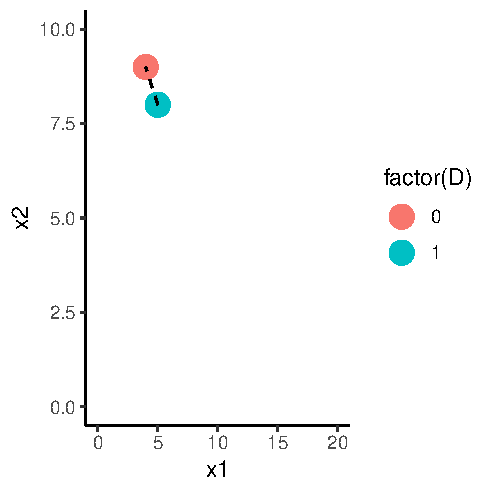
\includegraphics[width=\maxwidth]{figure/unnamed-chunk-3-1} 

\end{knitrout}
\end{frame}

\begin{frame}
\frametitle{Matching}
\begin{itemize}
\item Matching \textit{always} produces a smaller dataset
\pause
\begin{itemize}
\item So there is a trade-off between improving balance and retaining a large sample
\end{itemize}
\pause
\item After matching, for the analysis we can either:
\begin{enumerate}
\item Calculate the difference in means between treated and control groups
\pause
\item Conduct the normal regression: $Y \sim D$
\begin{itemize}
\item Option to include all our matching variables as controls
\item This will help control for any \textbf{residual imbalance} (esp. for continuous variables)
\end{itemize}
\end{enumerate}
\end{itemize}
\end{frame}

\begin{frame}
\frametitle{Matching}
\begin{itemize}
\item Which variables to match on?
\pause
\begin{itemize}
\item Treatment variable? \pause \textbf{No!} We need treated and control units who are both male
\pause
\item Outcome variable? \pause \textbf{No!} That's selecting on the dependent variable - biased!
\pause
\item Post-treatment variables? \pause \textbf{No!} This will bias our causal effect, just as in regression
\pause
\item Pre-treatment Confounders? \pause \textbf{Yes!} We want to remove imbalance due to confounders 
\end{itemize}
\end{itemize}
\end{frame}

\setbeamercolor{background canvas}{bg=}
\includepdf[pages={13-18}]{Ho_Slides.pdf}

\begin{frame}
\frametitle{Matching}
\begin{itemize}
\item To identify 'close' matches we need some measure of distance between units' covariates
\pause
\end{itemize}
\begin{enumerate}
\item Matching on few categorical variables: \textbf{Exact Matching}
\pause
\item Matching on continuous variables (sequential): \textbf{Nearest-Neighbour Matching}
\pause
\item Matching to maximize balance: \textbf{Optimal/Genetic Matching}
\pause
\item Matching on the probability of treatment: \textbf{Propensity Score Matching}
\end{enumerate}
\end{frame}

\section{Alternative Matching Methods}



\begin{frame}
\frametitle{Exact Matching}
\begin{center}
\begin{knitrout}
\definecolor{shadecolor}{rgb}{0.969, 0.969, 0.969}\color{fgcolor}
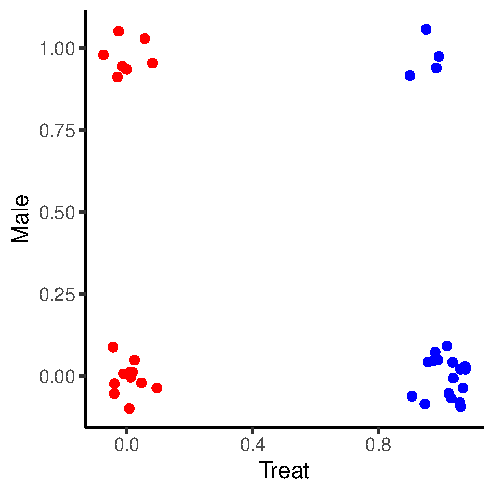
\includegraphics[width=\maxwidth]{figure/exact_matching_1-1} 

\end{knitrout}
\end{center}
\end{frame}

\begin{frame}
\frametitle{Exact Matching}
\begin{center}
\begin{knitrout}
\definecolor{shadecolor}{rgb}{0.969, 0.969, 0.969}\color{fgcolor}
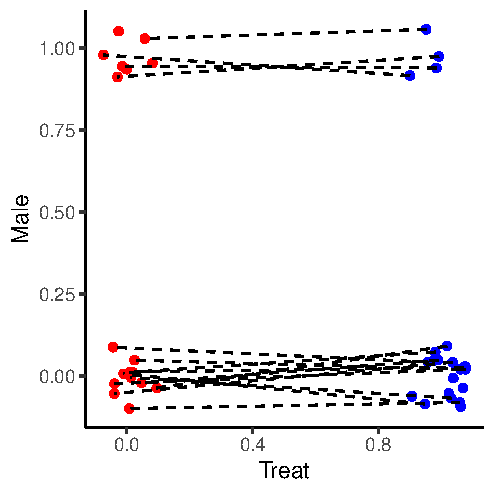
\includegraphics[width=\maxwidth]{figure/exact_matching_2a-1} 

\end{knitrout}
\end{center}
\end{frame}

\begin{frame}
\frametitle{Exact Matching}
\begin{center}
\begin{knitrout}
\definecolor{shadecolor}{rgb}{0.969, 0.969, 0.969}\color{fgcolor}
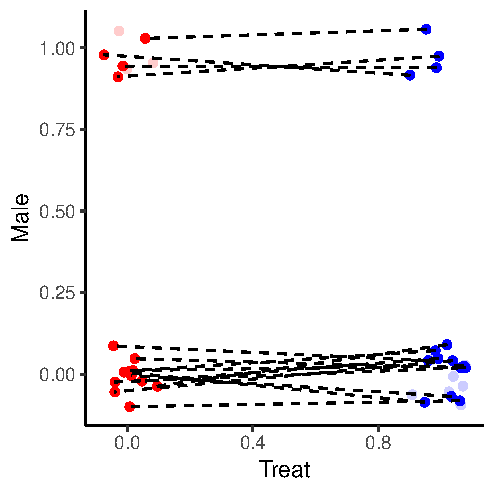
\includegraphics[width=\maxwidth]{figure/exact_matching_2b-1} 

\end{knitrout}
\end{center}
\end{frame}

\begin{frame}
\frametitle{Exact Matching}
\begin{center}
\begin{knitrout}
\definecolor{shadecolor}{rgb}{0.969, 0.969, 0.969}\color{fgcolor}
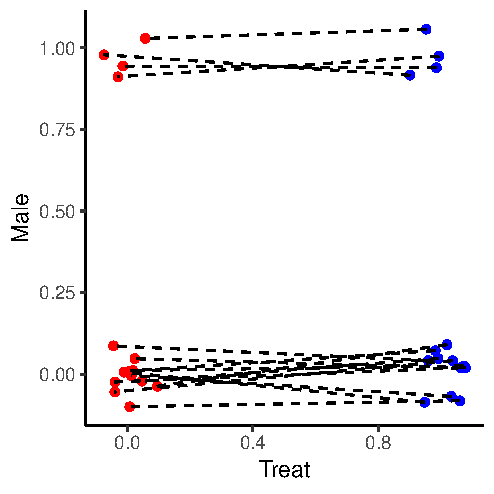
\includegraphics[width=\maxwidth]{figure/exact_matching_3-1} 

\end{knitrout}
\end{center}
\end{frame}

\begin{frame}
\frametitle{Exact Matching}
\begin{itemize}
\item Exact matching defines clear counterfactuals:
\begin{itemize}
\item What is the difference in the outcome between treated and control units \textbf{for units of the same gender}
\pause
\end{itemize}
\item After matching, we \textbf{prune/remove} unmatched units
\pause
\item \textbf{Then delete the link between the paired units, we don't need it any more}
\pause
\item Then compare the outcome of the \textbf{remaining} treated and control units
\pause
\begin{itemize}
\item Difference in means
\pause
\item Or regression of outcome on treatment
\end{itemize}
\end{itemize}
\end{frame}

\begin{frame}
\frametitle{Exact Matching}
\begin{center}
% latex table generated in R 3.6.0 by xtable 1.8-4 package
% Thu May 30 13:41:56 2019
\begin{table}[ht]
\centering
\begin{tabular}{rlrrr}
  \hline
 & Units & Means Treated & Means Control & Mean Diff \\ 
  \hline
1 & All & 0.18 & 0.39 & -0.21 \\ 
  2 & Matched & 0.27 & 0.27 & 0.00 \\ 
   \hline
\end{tabular}
\end{table}

\end{center}
\end{frame}

\begin{frame}
\frametitle{Exact Matching Analysis}
\begin{center}
\begin{knitrout}
\definecolor{shadecolor}{rgb}{0.969, 0.969, 0.969}\color{fgcolor}
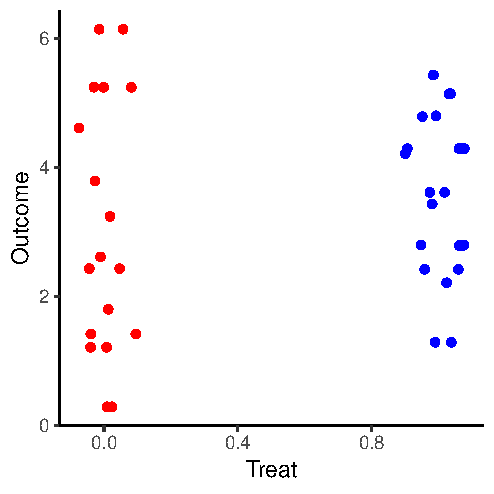
\includegraphics[width=\maxwidth]{figure/exact_matching_analysis0-1} 

\end{knitrout}
\end{center}
\end{frame}

\begin{frame}
\frametitle{Exact Matching Analysis}
\begin{center}
\begin{knitrout}
\definecolor{shadecolor}{rgb}{0.969, 0.969, 0.969}\color{fgcolor}
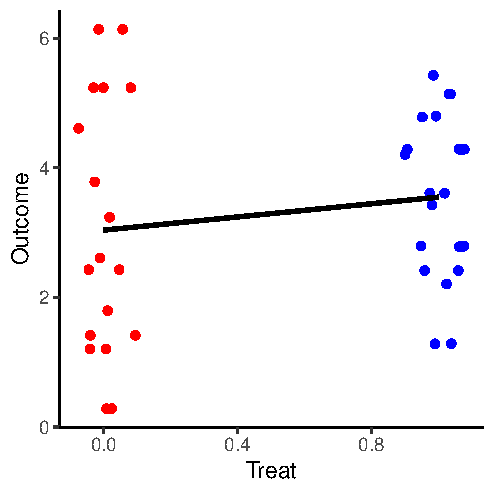
\includegraphics[width=\maxwidth]{figure/exact_matching_analysis0b-1} 

\end{knitrout}
\end{center}
\end{frame}

\begin{frame}
\frametitle{Exact Matching Analysis}
\begin{center}
\begin{knitrout}
\definecolor{shadecolor}{rgb}{0.969, 0.969, 0.969}\color{fgcolor}
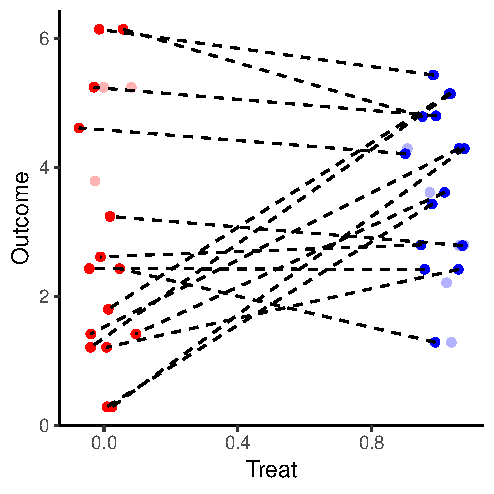
\includegraphics[width=\maxwidth]{figure/exact_matching_analysis-1} 

\end{knitrout}
\end{center}
\end{frame}

\begin{frame}
\frametitle{Exact Matching Analysis}
\begin{center}
\begin{knitrout}
\definecolor{shadecolor}{rgb}{0.969, 0.969, 0.969}\color{fgcolor}
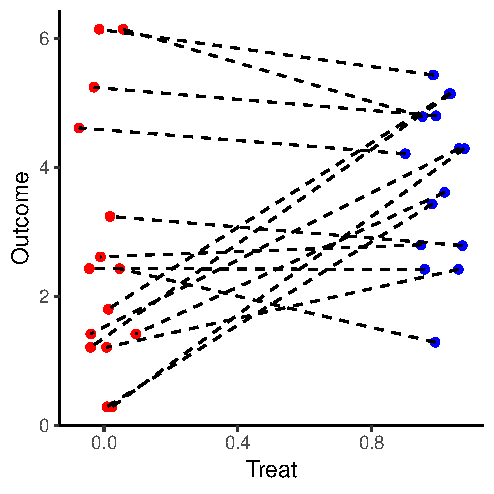
\includegraphics[width=\maxwidth]{figure/exact_matching_analysis1b-1} 

\end{knitrout}
\end{center}
\end{frame}

\begin{frame}
\frametitle{Exact Matching Analysis}
\begin{center}
\begin{knitrout}
\definecolor{shadecolor}{rgb}{0.969, 0.969, 0.969}\color{fgcolor}
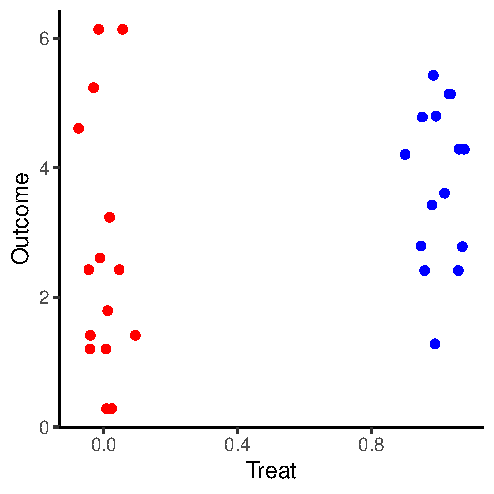
\includegraphics[width=\maxwidth]{figure/exact_matching_analysis2-1} 

\end{knitrout}
\end{center}
\end{frame}

\begin{frame}
\frametitle{Exact Matching Analysis}
\begin{center}
\begin{knitrout}
\definecolor{shadecolor}{rgb}{0.969, 0.969, 0.969}\color{fgcolor}
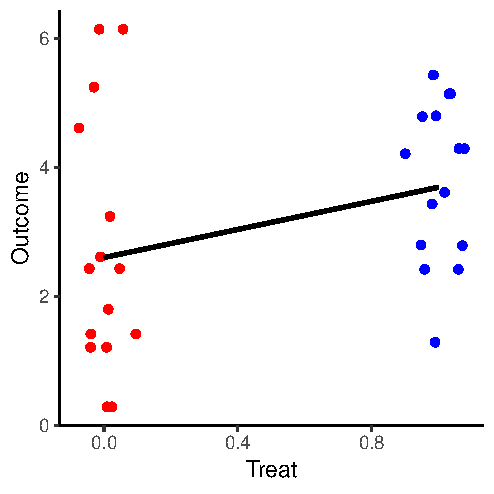
\includegraphics[width=\maxwidth]{figure/exact_matching_analysis3-1} 

\end{knitrout}
\end{center}
\end{frame}

\begin{frame}
\frametitle{Exact Matching Analysis}
\begin{center}
\begin{knitrout}
\definecolor{shadecolor}{rgb}{0.969, 0.969, 0.969}\color{fgcolor}
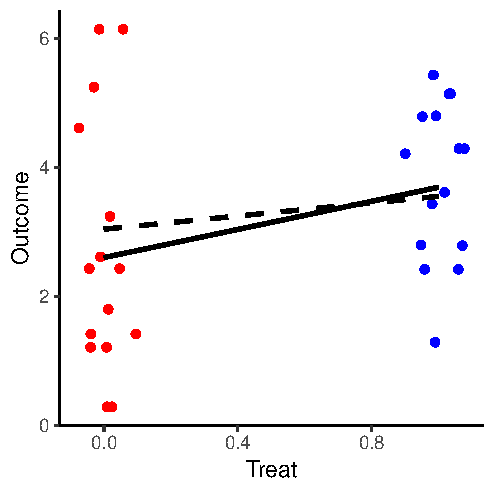
\includegraphics[width=\maxwidth]{figure/exact_matching_analysis4-1} 

\end{knitrout}
\end{center}
\end{frame}



\begin{frame}
\frametitle{Nearest Neighbour Matching}
\begin{center}
\begin{knitrout}
\definecolor{shadecolor}{rgb}{0.969, 0.969, 0.969}\color{fgcolor}
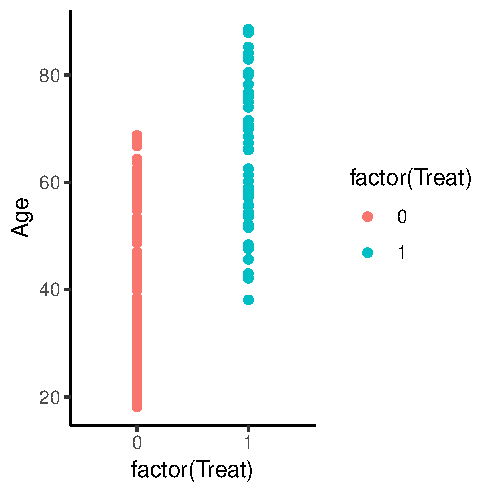
\includegraphics[width=\maxwidth]{figure/nearest_matching_1-1} 

\end{knitrout}
\end{center}
\end{frame}

\begin{frame}
\frametitle{Nearest Neighbour Matching}
\begin{center}
\begin{knitrout}
\definecolor{shadecolor}{rgb}{0.969, 0.969, 0.969}\color{fgcolor}
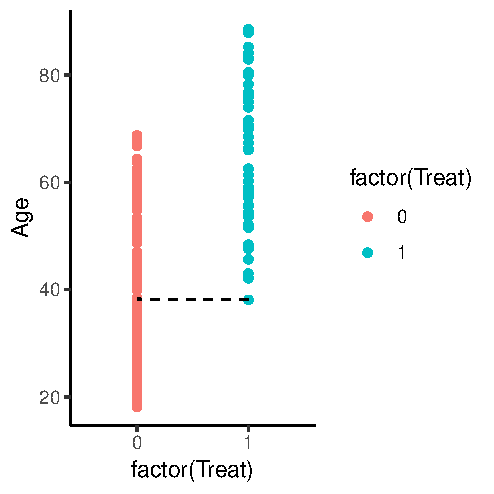
\includegraphics[width=\maxwidth]{figure/nearest_matching_2_pre-1} 

\end{knitrout}
\end{center}
\end{frame}


\begin{frame}
\frametitle{Nearest Neighbour Matching}
\begin{center}
\begin{knitrout}
\definecolor{shadecolor}{rgb}{0.969, 0.969, 0.969}\color{fgcolor}
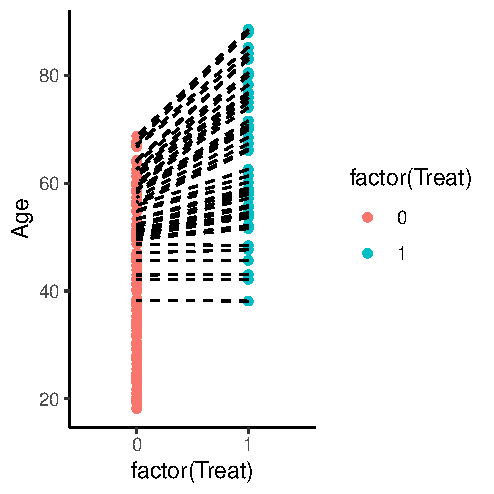
\includegraphics[width=\maxwidth]{figure/nearest_matching_2-1} 

\end{knitrout}
\end{center}
\end{frame}

\begin{frame}
\frametitle{Nearest Neighbour Matching}
\begin{center}
\begin{knitrout}
\definecolor{shadecolor}{rgb}{0.969, 0.969, 0.969}\color{fgcolor}
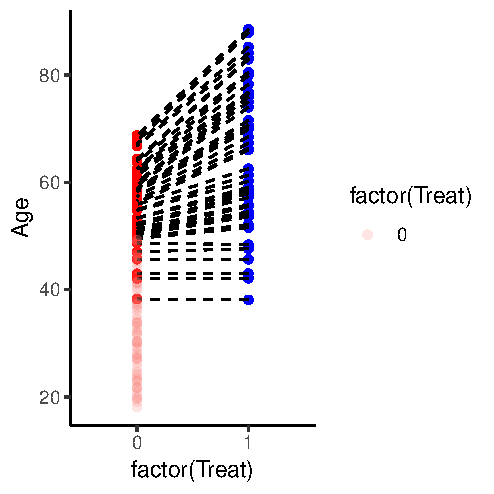
\includegraphics[width=\maxwidth]{figure/nearest_matching_3-1} 

\end{knitrout}
\end{center}
\end{frame}

\begin{frame}
\frametitle{Nearest Neighbour Matching}
\begin{center}
\begin{knitrout}
\definecolor{shadecolor}{rgb}{0.969, 0.969, 0.969}\color{fgcolor}
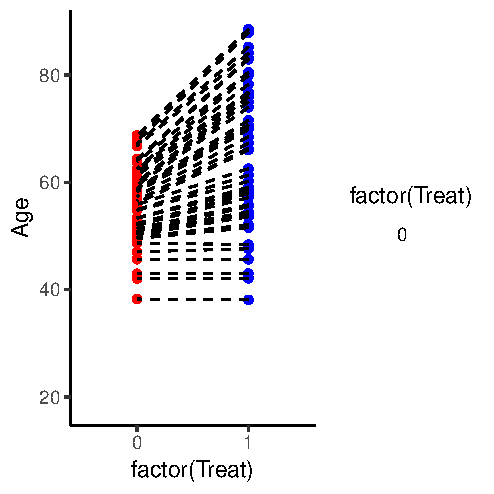
\includegraphics[width=\maxwidth]{figure/nearest_matching_4-1} 

\end{knitrout}
\end{center}
\end{frame}

\begin{frame}
\frametitle{Nearest Neighbour Matching}
\begin{center}
% latex table generated in R 3.6.0 by xtable 1.8-4 package
% Thu May 30 13:42:02 2019
\begin{table}[ht]
\centering
\begin{tabular}{rlrrr}
  \hline
 & Units & Means Treated & Means Control & Mean Diff \\ 
  \hline
1 & All & 65.70 & 42.67 & 23.03 \\ 
  2 & Matched & 65.70 & 56.09 & 9.61 \\ 
   \hline
\end{tabular}
\end{table}

\end{center}
\end{frame}




\begin{frame}
\frametitle{Nearest Neighbour Matching}
\begin{itemize}
\item Two potential problems with nearest neighbour matching:
\pause
\begin{enumerate}
\item \textbf{Nearest does not mean close:} The oldest treated units are matched with, but very different to, the oldest control units
\pause
\begin{itemize}
\item We need some \textbf{absolute} limits on the distance we can match units within
\pause
\item We can add 'calipers' to matching to match only within a fixed range
\pause
\end{itemize}
\item \textbf{The order of matching matters:} The first matches use up units that might make better matches for later treated units
\pause
\begin{itemize}
\item To maximize balance we need to 'look ahead' and match in the right order
\pause
\item For this we can use optimal or genetic matching, which is fully automated
\end{itemize}
\end{enumerate}
\end{itemize}
\end{frame}



\begin{frame}
\frametitle{Nearest Neighbour Matching with Caliper}
\begin{center}
\begin{knitrout}
\definecolor{shadecolor}{rgb}{0.969, 0.969, 0.969}\color{fgcolor}
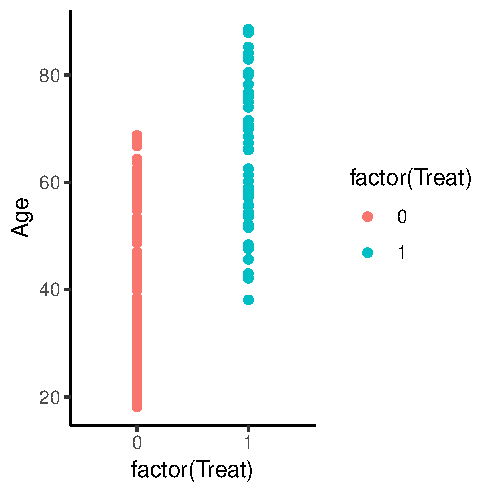
\includegraphics[width=\maxwidth]{figure/nearest_matching_1_caliper-1} 

\end{knitrout}
\end{center}
\end{frame}

\begin{frame}
\frametitle{Nearest Neighbour Matching with Caliper}
\begin{center}
\begin{knitrout}
\definecolor{shadecolor}{rgb}{0.969, 0.969, 0.969}\color{fgcolor}
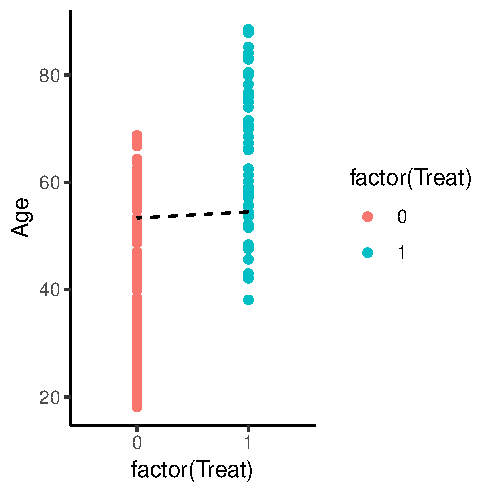
\includegraphics[width=\maxwidth]{figure/nearest_matching_2_pre_caliper-1} 

\end{knitrout}
\end{center}
\end{frame}

\begin{frame}
\frametitle{Nearest Neighbour Matching with Caliper}
\begin{center}
\begin{knitrout}
\definecolor{shadecolor}{rgb}{0.969, 0.969, 0.969}\color{fgcolor}
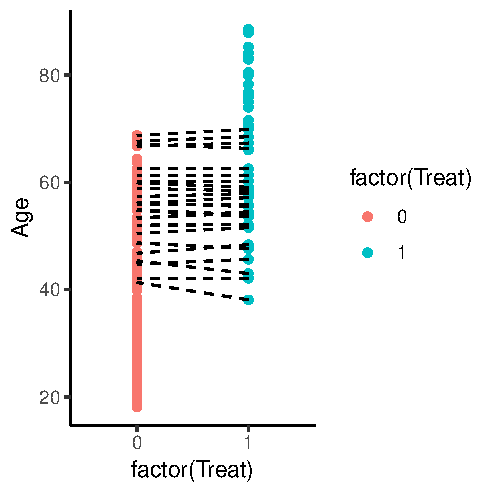
\includegraphics[width=\maxwidth]{figure/nearest_matching_2_caliper-1} 

\end{knitrout}
\end{center}
\end{frame}

\begin{frame}
\frametitle{Nearest Neighbour Matching with Caliper}
\begin{center}
\begin{knitrout}
\definecolor{shadecolor}{rgb}{0.969, 0.969, 0.969}\color{fgcolor}
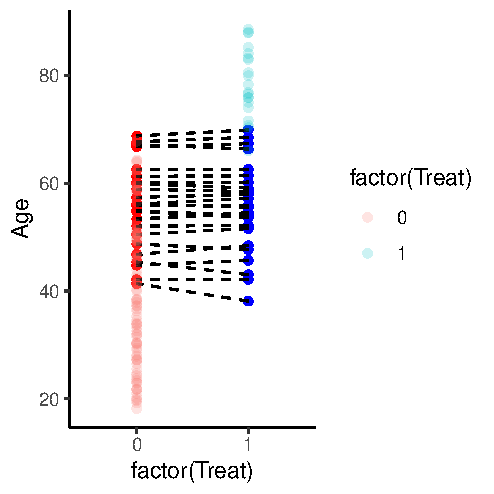
\includegraphics[width=\maxwidth]{figure/nearest_matching_3_caliper-1} 

\end{knitrout}
\end{center}
\end{frame}

\begin{frame}
\frametitle{Nearest Neighbour Matching with Caliper}
\begin{center}
\begin{knitrout}
\definecolor{shadecolor}{rgb}{0.969, 0.969, 0.969}\color{fgcolor}
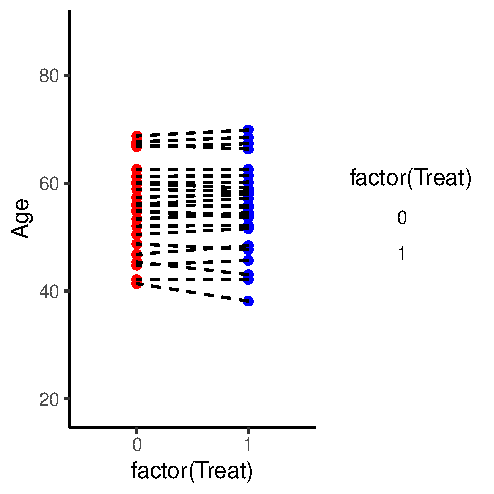
\includegraphics[width=\maxwidth]{figure/nearest_matching_4_caliper-1} 

\end{knitrout}
\end{center}
\end{frame}

\begin{frame}
\frametitle{Nearest Neighbour Matching with Caliper}
\begin{center}
% latex table generated in R 3.6.0 by xtable 1.8-4 package
% Thu May 30 13:42:05 2019
\begin{table}[ht]
\centering
\begin{tabular}{rlrrr}
  \hline
 & Units & Means Treated & Means Control & Mean Diff \\ 
  \hline
1 & All & 65.70 & 42.67 & 23.03 \\ 
  2 & Matched & 55.41 & 55.46 & -0.06 \\ 
   \hline
\end{tabular}
\end{table}

\end{center}
\begin{itemize}
\item Note: p-values don't mean so much for balance tests
\pause
\item We always want to improve balance as much as possible
\pause
\item Better to compare (standardized) difference in means
\end{itemize}
\end{frame}



\begin{frame}
\frametitle{Optimal Matching}
\begin{center}
\begin{knitrout}
\definecolor{shadecolor}{rgb}{0.969, 0.969, 0.969}\color{fgcolor}
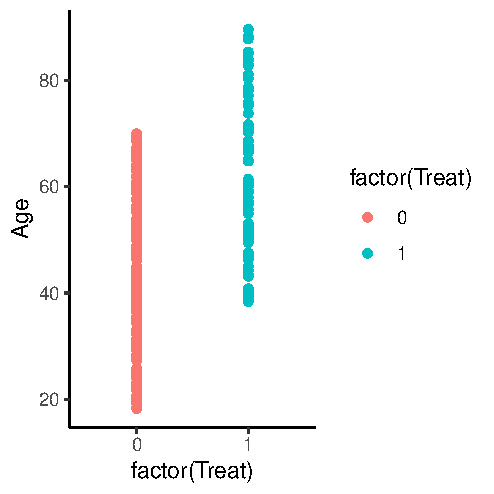
\includegraphics[width=\maxwidth]{figure/optimal_matching_1-1} 

\end{knitrout}
\end{center}
\end{frame}

\begin{frame}
\frametitle{Optimal Matching}
\begin{center}
\begin{knitrout}
\definecolor{shadecolor}{rgb}{0.969, 0.969, 0.969}\color{fgcolor}
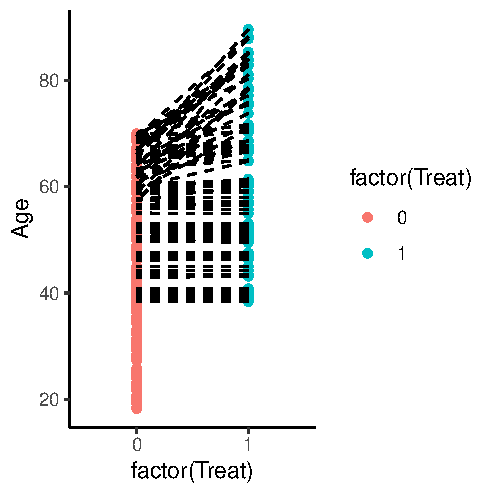
\includegraphics[width=\maxwidth]{figure/optimal_matching_2-1} 

\end{knitrout}
\end{center}
\end{frame}

\begin{frame}
\frametitle{Optimal Matching}
\begin{center}
\begin{knitrout}
\definecolor{shadecolor}{rgb}{0.969, 0.969, 0.969}\color{fgcolor}
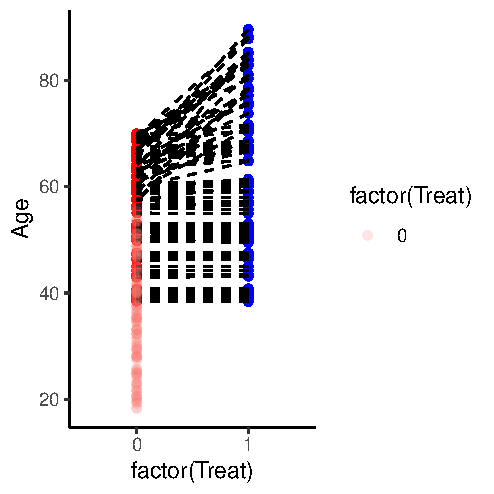
\includegraphics[width=\maxwidth]{figure/optimal_matching_3-1} 

\end{knitrout}
\end{center}
\end{frame}

\begin{frame}
\frametitle{Optimal Matching}
\begin{center}
\begin{knitrout}
\definecolor{shadecolor}{rgb}{0.969, 0.969, 0.969}\color{fgcolor}
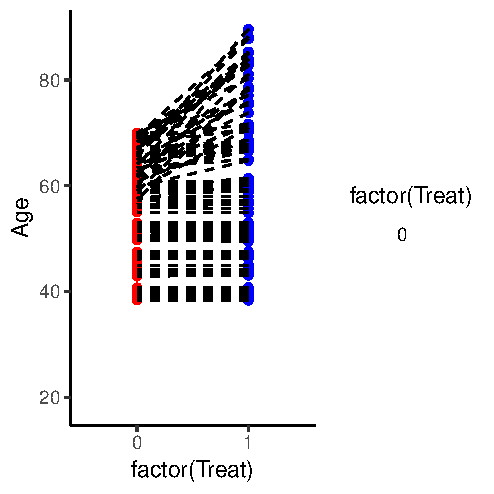
\includegraphics[width=\maxwidth]{figure/optimal_matching_4-1} 

\end{knitrout}
\end{center}
\end{frame}

\begin{frame}
\frametitle{Optimal Matching}
\begin{center}
% latex table generated in R 3.6.0 by xtable 1.8-4 package
% Thu May 30 13:42:09 2019
\begin{table}[ht]
\centering
\begin{tabular}{rlrrr}
  \hline
 & Units & Means Treated & Means Control & Mean Diff \\ 
  \hline
1 & All & 62.60 & 44.64 & 17.96 \\ 
  2 & Matched & 62.60 & 57.57 & 5.03 \\ 
   \hline
\end{tabular}
\end{table}

\end{center}
\end{frame}



\begin{frame}
\frametitle{Propensity Score Matching}
\begin{itemize}
\item With many covariates we have a dimensionality challenge
\pause
\begin{itemize}
\item Overlap is almost zero
\pause
\item Counterfactuals are impossible to define
\end{itemize}
\item The propensity score collapses matching to a single dimension
\pause
\begin{itemize}
\item Confounders only matter to the extent they affect treatment
\pause
\item So let's use the confounders to \textbf{predict treatment}
\pause
\item That's different to actual treatment status, with the remainder due to 'random' factors (if we include all confounders)
\pause
\end{itemize}
\item Then use the propensity score (probability 0-1) to match treated and control units which have the same ex ante probability of treatment
\end{itemize}
\end{frame}

\begin{frame}
\frametitle{Propensity Score Matching}
\begin{itemize}
\item But some concerns about drawbacks of propensity score matching
\pause
\item May have poor balance on individual confounders
\pause
\item Balance may get worse as we remove more units
\pause
\item We have to get the functional form of the treatment explanation right (linear, quadratic etc.) so we remain vulnerable to model dependence!
\end{itemize}
\end{frame}

\begin{frame}
\frametitle{Propensity Score Matching}
\begin{itemize}
\item Treatment: 1/0
\item Confounder: Age
\item Logit model predicting treatment:
\end{itemize}
$$Treat_i = \alpha + \beta Age_i +\epsilon_i$$
\pause
$$Predicted\_Treat_i = -7.19 + 0.116 Age_i +\epsilon_i$$
\pause
\begin{itemize}
\item Match on the values of $Predicted\_Treat_i$ (fitted values of the regression)
\pause
\item I.e. match units with a similar \textit{probability} of treatment
\pause
\item ...Regardless of whether they actually get treated
\end{itemize}
\end{frame}

\begin{frame}
\frametitle{Propensity Score Matching}
\begin{center}
\begin{knitrout}
\definecolor{shadecolor}{rgb}{0.969, 0.969, 0.969}\color{fgcolor}
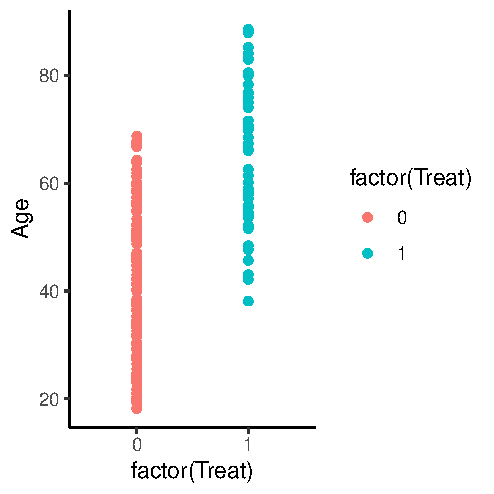
\includegraphics[width=\maxwidth]{figure/pscore_matching_1-1} 

\end{knitrout}
\end{center}
\end{frame}

\begin{frame}
\frametitle{Propensity Score Matching}
\begin{center}
\begin{knitrout}
\definecolor{shadecolor}{rgb}{0.969, 0.969, 0.969}\color{fgcolor}
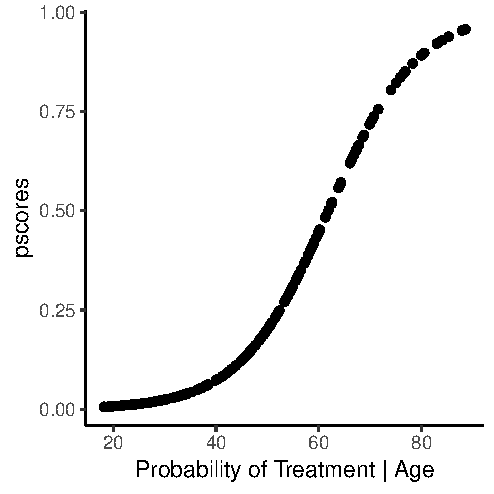
\includegraphics[width=\maxwidth]{figure/pscore_matching_2-1} 

\end{knitrout}
\end{center}
\end{frame}

\begin{frame}
\frametitle{Propensity Score Matching}
\begin{center}
\begin{knitrout}
\definecolor{shadecolor}{rgb}{0.969, 0.969, 0.969}\color{fgcolor}
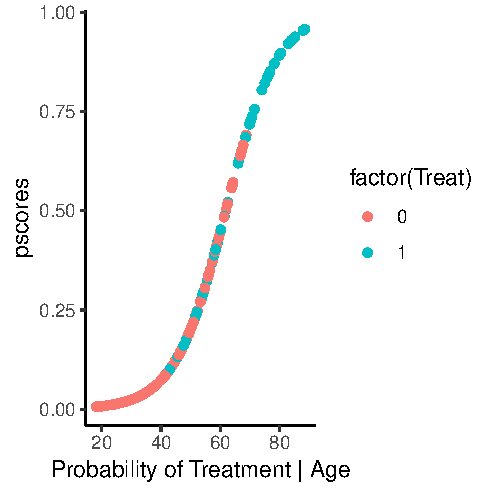
\includegraphics[width=\maxwidth]{figure/pscore_matching_3-1} 

\end{knitrout}
\end{center}
\end{frame}

\begin{frame}
\frametitle{Propensity Score Matching}
\begin{center}
\begin{knitrout}
\definecolor{shadecolor}{rgb}{0.969, 0.969, 0.969}\color{fgcolor}
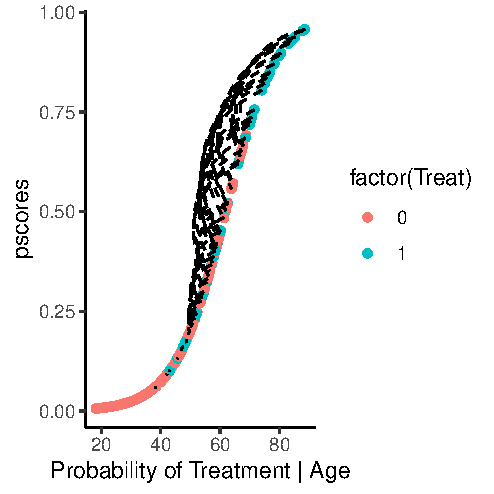
\includegraphics[width=\maxwidth]{figure/pscore_matching_4-1} 

\end{knitrout}
\end{center}
\end{frame}

\begin{frame}
\frametitle{Propensity Score Matching}
\begin{center}
\begin{knitrout}
\definecolor{shadecolor}{rgb}{0.969, 0.969, 0.969}\color{fgcolor}
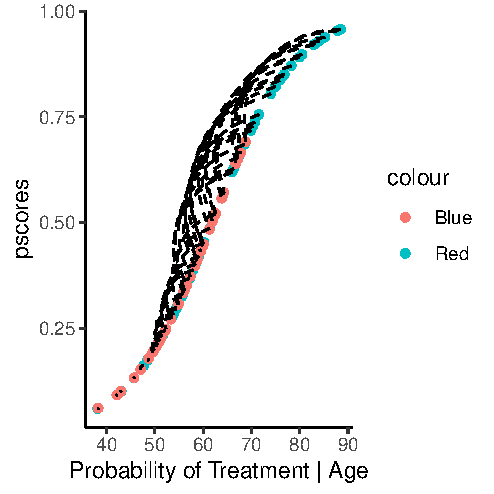
\includegraphics[width=\maxwidth]{figure/pscore_matching_5-1} 

\end{knitrout}
\end{center}
\end{frame}

\begin{frame}
\frametitle{Propensity Score Matching}
\begin{center}
% latex table generated in R 3.6.0 by xtable 1.8-4 package
% Thu May 30 13:42:13 2019
\begin{table}[ht]
\centering
\begin{tabular}{rlrrr}
  \hline
 & Units & Means Treated & Means Control & Mean Diff \\ 
  \hline
1 & All & 0.57 & 0.18 & 0.39 \\ 
  2 & Matched & 0.57 & 0.36 & 0.21 \\ 
   \hline
\end{tabular}
\end{table}

\end{center}
\end{frame}



\begin{frame}
\frametitle{Propensity Score Matching with Caliper}
\begin{center}
\begin{knitrout}
\definecolor{shadecolor}{rgb}{0.969, 0.969, 0.969}\color{fgcolor}
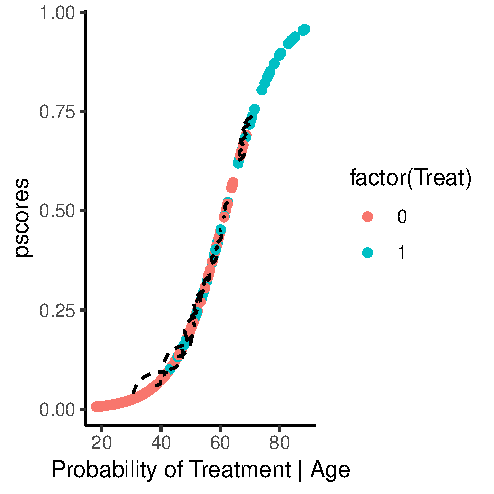
\includegraphics[width=\maxwidth]{figure/pscore_matching_caliper_1-1} 

\end{knitrout}
\end{center}
\end{frame}

\begin{frame}
\frametitle{Propensity Score Matching with Caliper}
\begin{center}
\begin{knitrout}
\definecolor{shadecolor}{rgb}{0.969, 0.969, 0.969}\color{fgcolor}
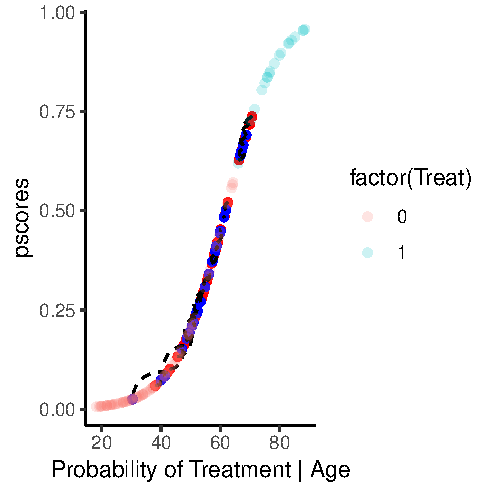
\includegraphics[width=\maxwidth]{figure/pscore_matching_caliper_2-1} 

\end{knitrout}
\end{center}
\end{frame}

\begin{frame}
\frametitle{Propensity Score Matching with Caliper}
\begin{center}
\begin{knitrout}
\definecolor{shadecolor}{rgb}{0.969, 0.969, 0.969}\color{fgcolor}
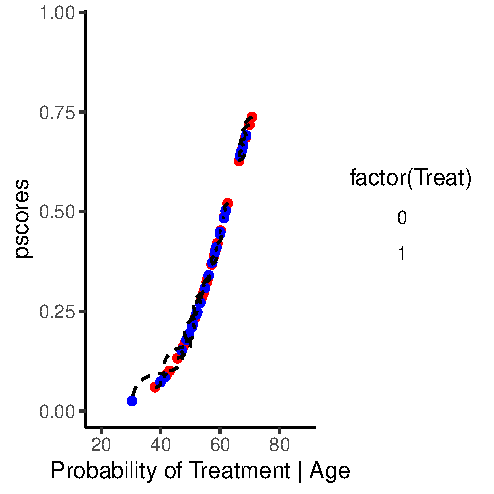
\includegraphics[width=\maxwidth]{figure/pscore_matching_caliper_3-1} 

\end{knitrout}
\end{center}
\end{frame}

\begin{frame}
\frametitle{Propensity Score Matching with Caliper}
\begin{center}
% latex table generated in R 3.6.0 by xtable 1.8-4 package
% Thu May 30 13:42:14 2019
\begin{table}[ht]
\centering
\begin{tabular}{rlrrr}
  \hline
 & Units & Means Treated & Means Control & Mean Diff \\ 
  \hline
1 & All & 0.57 & 0.18 & 0.39 \\ 
  2 & Matched & 0.36 & 0.35 & 0.01 \\ 
   \hline
\end{tabular}
\end{table}

\end{center}
\end{frame}

\begin{frame}
\frametitle{Matching}
\begin{itemize}
\item Matching was supposed to be 'non-parametric' to reduce researcher influence, but there are a lot of options here!
\pause
\item That's okay! Regression has no measure of 'success', but with matching we want to maximize balance
\pause
\begin{itemize}
\item \textbf{Without} looking at the outcome variables
\end{itemize}
\pause
\item How much trimming/pruning should we undertake?
\pause
\item We can always enforce \textbf{stricter} matching (eg. narrower calipers, more exact matching) to get better balance
\pause
\item But our N will approach zero, so little statistical power
\pause
\item A Bias-variance trade-off
\pause
\item Try alternative specifications
\end{itemize}
\end{frame}

\begin{frame}
\frametitle{Matching}
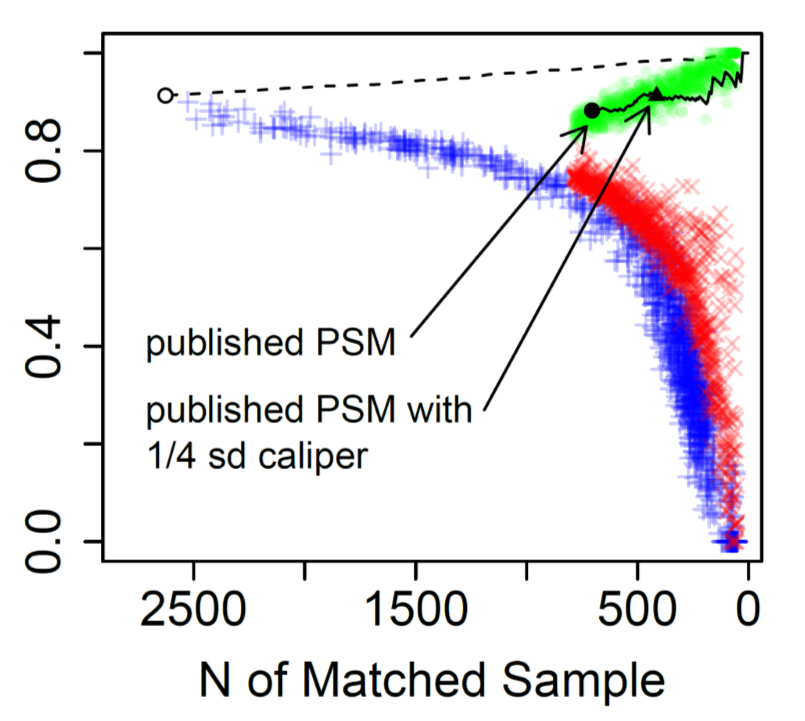
\includegraphics[width=0.58\textwidth]{Balance-N_trade-off.png}
\end{frame}

\begin{frame}
\frametitle{Matching}
\begin{itemize}
\item Matching preferred to regression where:
\pause
\begin{itemize}
\item Never! Do both!
\end{itemize}
\item Matching makes a big contribution where there's poor overlap
\pause
\item Matching + Regression = "Doubly Robust"
\pause
\begin{itemize}
\item If \textbf{either} matching produces balance \textbf{OR} we have the correct functional form for regression, we can make causal inference
\end{itemize}
\end{itemize}
\end{frame}

\section{Matching vs. Experiments}

\begin{frame}
\frametitle{Matching}
\begin{itemize}
\item Arceneaux, Gerber and Green (2005)
\pause
\item How does matching work on experimental (IV) data? (eg. for how to get voters to vote)
\pause
\item Matching is biased compared to the experimental results
\pause
\item Lots of controls 
\pause
\item But unobserved confounders mean matching can't recover causal estimates
\end{itemize}
\end{frame}

\begin{frame}
\frametitle{Matching}
\begin{itemize}
\item Bias was due to whether people actually answered phone calls
\pause
\item Huge N, \textbf{Perfect balance}
\pause
\item Experimental measure: 0.4
\pause
\item OLS estimate: 2.7
\pause
\item Matching estimate: 2.8
\pause
\item We can't control for likelihood of answering the phone using the (many) covariates they have
\pause
\item Matching still relies on \textbf{measuring all confounders}
\end{itemize}
\end{frame}


\end{document}
